\section{Numerical experiments}\label{sec:numerical_experiments}

In this section, we report numerical experiments conducted with the Julia implementation of our algorithm, named TRAULLS\footnote{Trust Region AUgmented nonLinear Least-squares Solver}. All runs were performed with Julia 1.12.1 on a machine equipped with an Intel\textsuperscript{\textregistered} Core\textsuperscript{\texttrademark} Ultra 9  and 64 GiB of RAM. All the benchmarks we present here are also accessible in the \texttt{benchmark} folder of the GitHub repository.
The tests were carried out on a set of 52 constrained NLS problems from collections~\cite{hockschittkowski:1980, schittkowski:1987, lucksanvlcek:1999} and problems 2 and 3 referenced in~\cite{biegler-etal2000}. For problems with variable dimensions, we set the number of variables to $n \in \{100, 500, 1000\}$. Thus, we have a total of 82 problem instances ranging from 2 to 1001 variables, with up to 2994 residuals and 999 constraints. Problems with inequality constraints were converted to the form~\eqref{pb:cnls} by adding slack variables. For our tests, we set the criticality tolerance to $\omega_* = 10^{-5}$, the feasibility tolerance to $\eta_* = 10^{-6}$, the maximum number of outer iterations to 500 and the maximum number of inner iterations to 1000. The remaining parameters are set to $\mu_0 = 10$, $\tau = 100$, $\kappa_\omega = \beta_\omega = \eta = \omega = 1$, $\kappa_\eta = 0.1$, $\beta_\eta = 0.9$, $\kappa_{hyb} = 0.1$, $\delta_0 = 0.1$, and the trust-region constants $\alpha_1 = 0.25$, $\alpha_2 = 2.5$, $\eta_1 = 0.25$, $\eta_2 = 0.75$, $\gamma_1 = 0.0625$, in accordance with the conditions of Section~\ref{subsec:implementation_details}.

Since Julia compiles code on its first execution, a naive measurement would charge that compilation to the solver being timed, an overhead that does not amortize over a benchmark because each problem instantiates its own specialized code. To avoid this bias, and for all solvers considered in this section, each instance was solved once to warm up, the result of that first solve being discarded, then solved three times with the minimum of the three timings reported. We present our results with performance profiles of type Dolan--Mor\'e~\cite{dolanmore:2002} produced with the \texttt{BenchmarkProfiles.jl} package~\cite{benchmark-profiles-julia}.

\subsection{Comparison of Hessian approximations}\label{subsec:compare_hessians}

Our first set of experiments compares the behavior and performance of our algorithm depending on the Hessian approximation used during the inner minimization. We compared the GN approximation~\eqref{eq:hessian_gn_approx} against structured approximations of the form~\eqref{eq:hessian_full_approx}. Based on the structured secant equation~\eqref{eq:structured_secant_eq}, we implemented the SR1 update we discussed and the BFGS update that one can derive similarly. Both structured approximations were used in their plain and hybrid variants with the switching rule~\eqref{eq:hybrid_update_strategy}.

\subsubsection{Profiles on the whole test set}

We first compare these five strategies against three metrics: computation time, number of outer iterations and number of inner iterations. The last metric coincides with the number of residual evaluations, since the trust-region mechanism evaluates the residuals exactly once per inner iteration. Results are reported in Figure~\ref{fig:compare_hessians}.

Two variants fail to reach a first-order critical point. The plain SR1 variant reaches the maximum number of outer iterations on problem HS373 and returns a point that is only feasible. The plain BFGS variant does the same on the instance of problem 5.1 from~\cite{lucksanvlcek:1999} with $n=500$, although it attains there the same value of the objective as the other variants. On three further instances -- HS23 and the instances with $n = 100$ of problems 5.13 and 5.14 from~\cite{lucksanvlcek:1999} -- all five variants converge, but the plain updates reach a local solution distinct from the one found by the GN and hybrid variants. Since a performance profile presupposes that all solvers address the same problem, these three instances are excluded from the profiles of this section, following the same relative-gap criterion as in Section~\ref{subsec:compare_solvers}. The profiles are therefore built on the remaining 79 instances, on which all five variants agree on the solution.

\begin{figure}[htbp]
	\centering
	\begin{subfigure}[b]{0.32\textwidth}
		\centering
		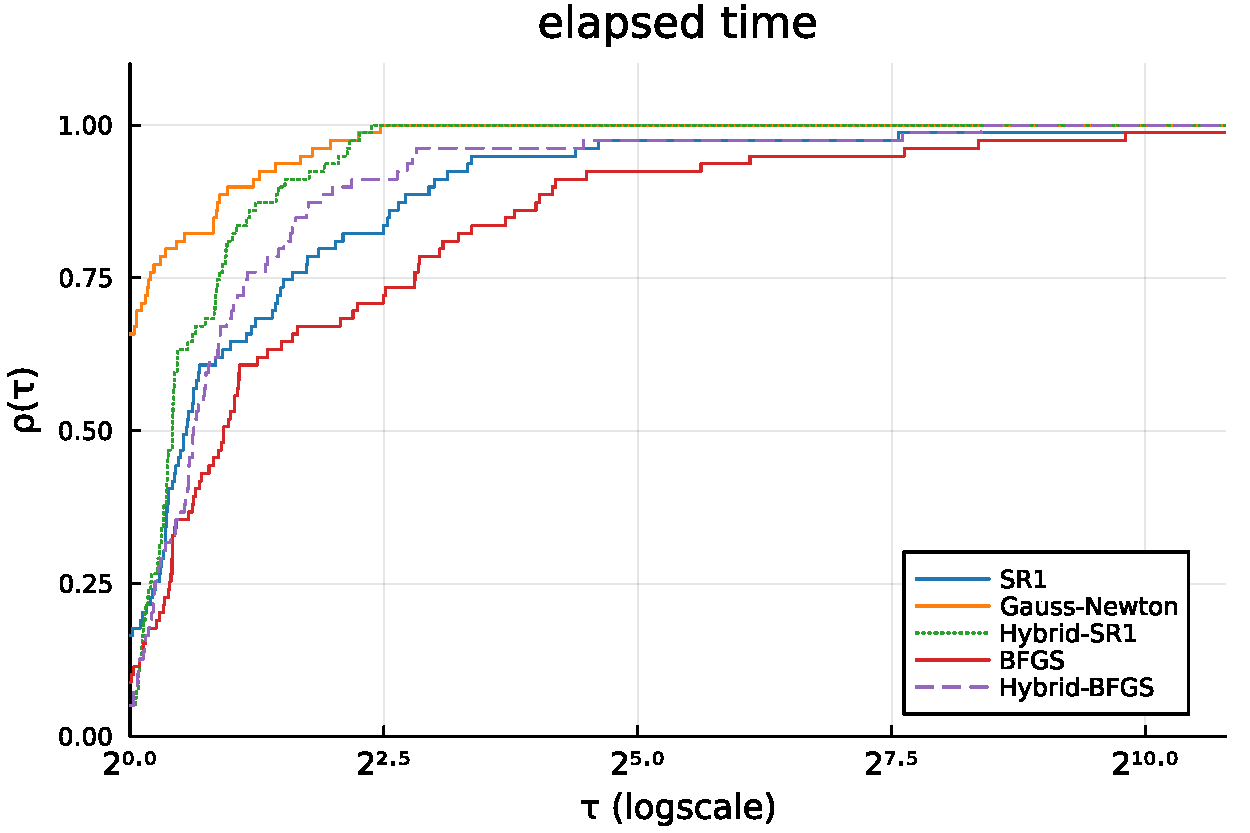
\includegraphics[width=\textwidth]{figures/fig1_traulls_variants_elapsed_time}
	\end{subfigure}
	\hfill
	\begin{subfigure}[b]{0.32\textwidth}
		\centering
		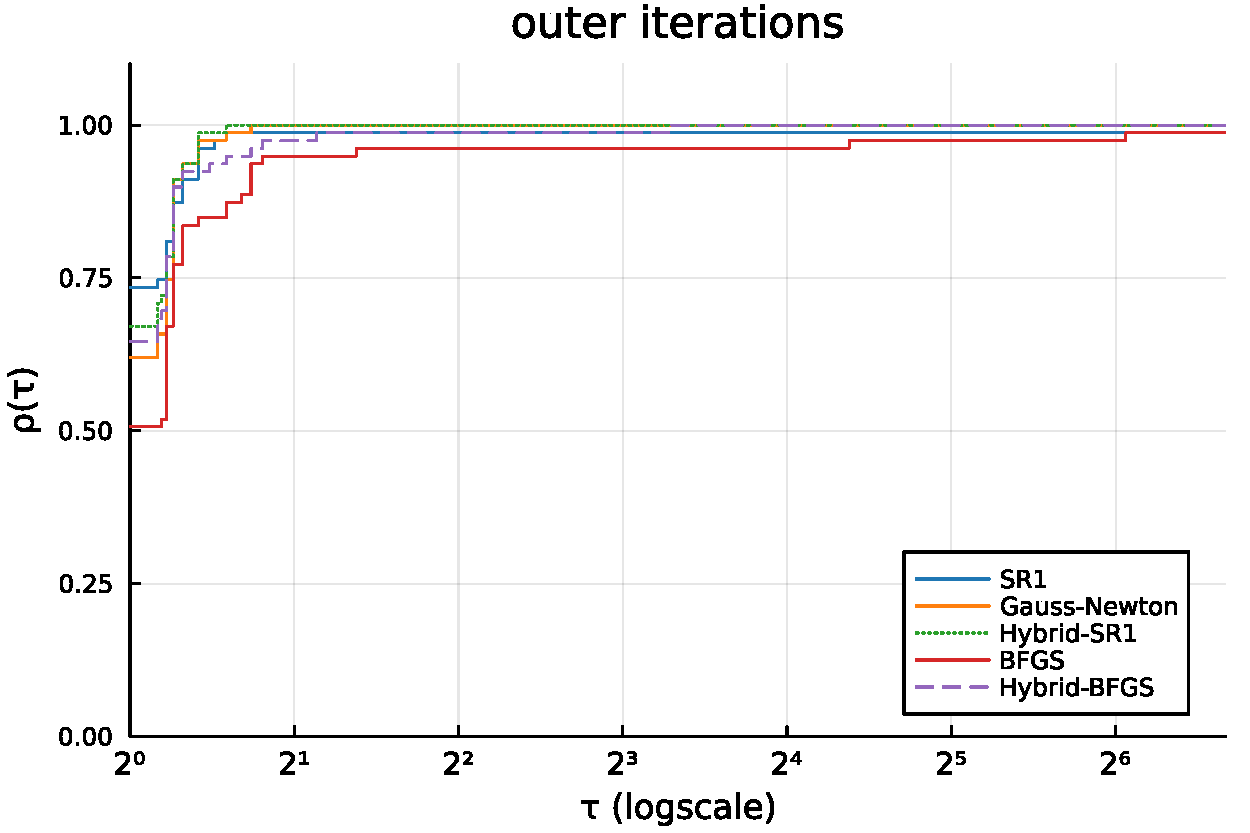
\includegraphics[width=\textwidth]{figures/fig3_traulls_variants_nouter_iter}
	\end{subfigure}
	\hfill
	\begin{subfigure}[b]{0.32\textwidth}
		\centering
		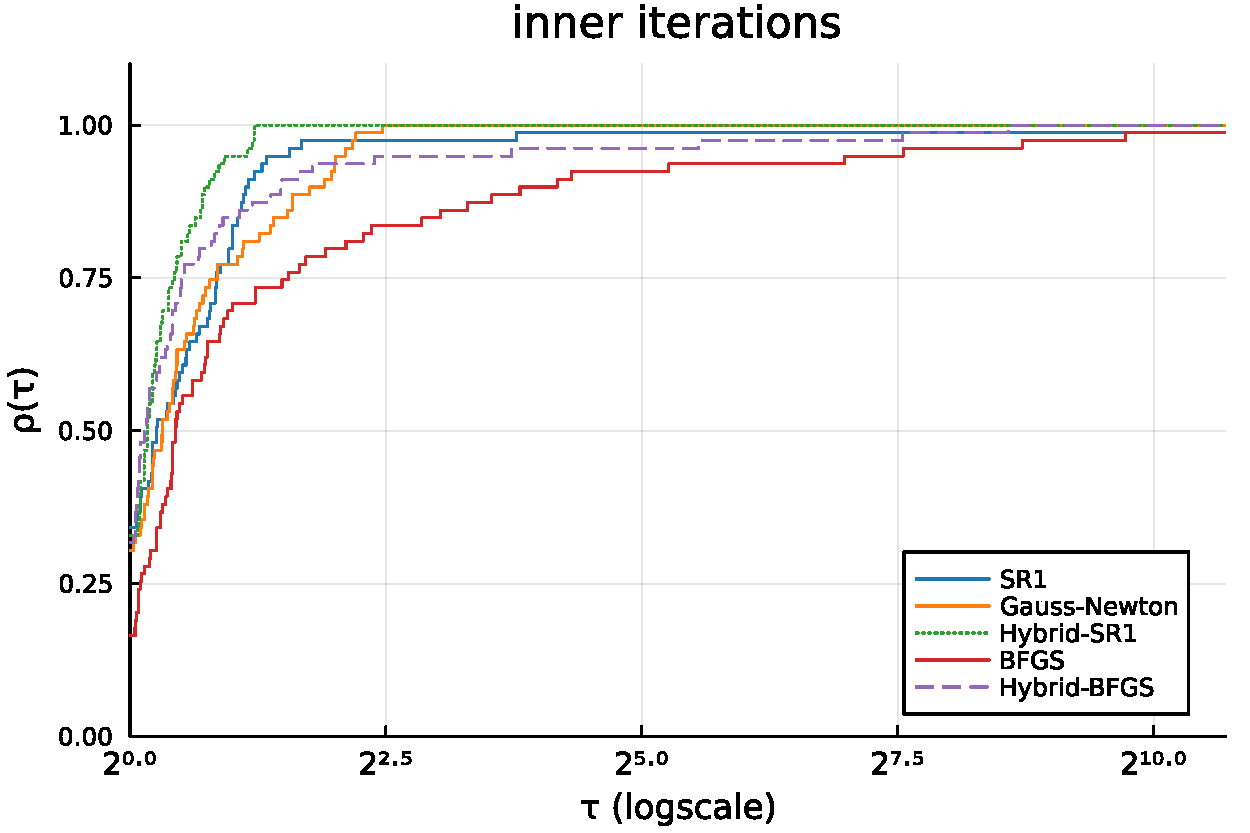
\includegraphics[width=\textwidth]{figures/fig2_traulls_variants_ninner_iter}
	\end{subfigure}
	\caption{Performance profiles comparing five different Hessian approximation strategies with respect to computation time (left), number of outer iterations (center),
		and number of inner iterations (right).}
	\label{fig:compare_hessians}
\end{figure}

In terms of computation time, the GN approximation is the fastest: it is the best strategy on 66\% of the instances and solves all of them within a factor 8 of the best time. Since it requires no additional storage or update computation, it is the cheapest per iteration as our method mainly involves matrix-vector products. The GN approximation especially dominates on problems having sparse Jacobians and small residuals at the solution, since the second-order terms are still stored as a dense matrix. The Hybrid-SR1 variant is a close second, within a factor $1.5$ of the best time on 65\% of the instances and within a factor 2 on 81\% of them.

The three metrics tell markedly different stories. Measured by outer iterations, the five strategies are almost indistinguishable: every variant except plain BFGS is within a factor $1.5$ of the best count on more than 98\% of the instances, which is expected since the outer loop is governed by the augmented Lagrangian updates rather than by the Hessian model. The number of inner iterations, on the other hand, separates them clearly. There, the hybrid variants outperform their plain counterparts and the GN approximation alike: Hybrid-SR1 is within a factor $1.25$ of the best count on 70\% of the instances and within a factor 2 on 95\% of them, against 52\% and 77\% for GN. These observations are consistent with the discussion about the hybrid switching rule~\eqref{eq:hybrid_update_strategy} which -- as in the unconstrained case -- correctly identifies situations where the Gauss--Newton approximation must be corrected and activates the structured quasi-Newton correction accordingly. Overall, Hybrid-SR1 appears to be the most robust variant, which also indicates that the SR1 approximation is well suited to handling negative curvature in the trust-region setting.

\subsubsection{Profiles stratified by residual magnitude at the solution}

To refine these observations and analyze separately the effectiveness of the approximated second-order correction and of the hybrid switching scheme, we stratify the previous profiles by the squared norm of the residuals at the solution, denoted $\|r_{opt}\|^2$. We distinguish four regimes: zero residuals ($\|r_{opt}\|^2 < 10^{-8}$, 18 instances), small residuals ($10^{-8} \le \|r_{opt}\|^2 < 1$, 17 instances), medium residuals ($1 \le \|r_{opt}\|^2 < 100$, 22 instances) and large residuals ($\|r_{opt}\|^2 \ge 100$, 22 instances). For this comparison, we retain the GN approximation and the SR1 update in its plain and hybrid variants. Figure~\ref{fig:stratified_reseval} reports the profiles on the number of residual evaluations -- equivalently, as discussed above, on the number of inner iterations -- and Figure~\ref{fig:stratified_time} those on computation time.

\begin{figure}[htbp]
	\centering
	\begin{subfigure}[b]{0.48\textwidth}
		\centering
		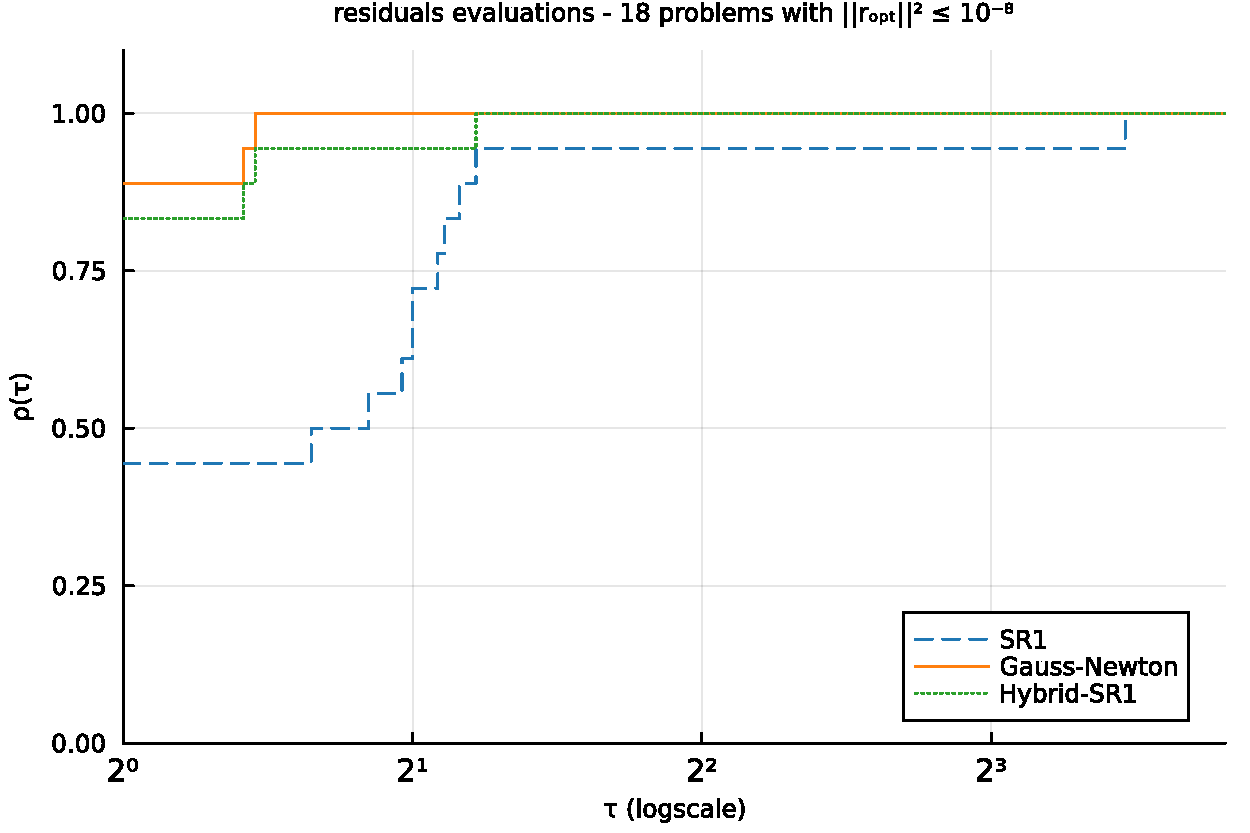
\includegraphics[width=\textwidth]{figures/fig8_zero_res_neval_residual}
	\end{subfigure}
	\hfill
	\begin{subfigure}[b]{0.48\textwidth}
		\centering
		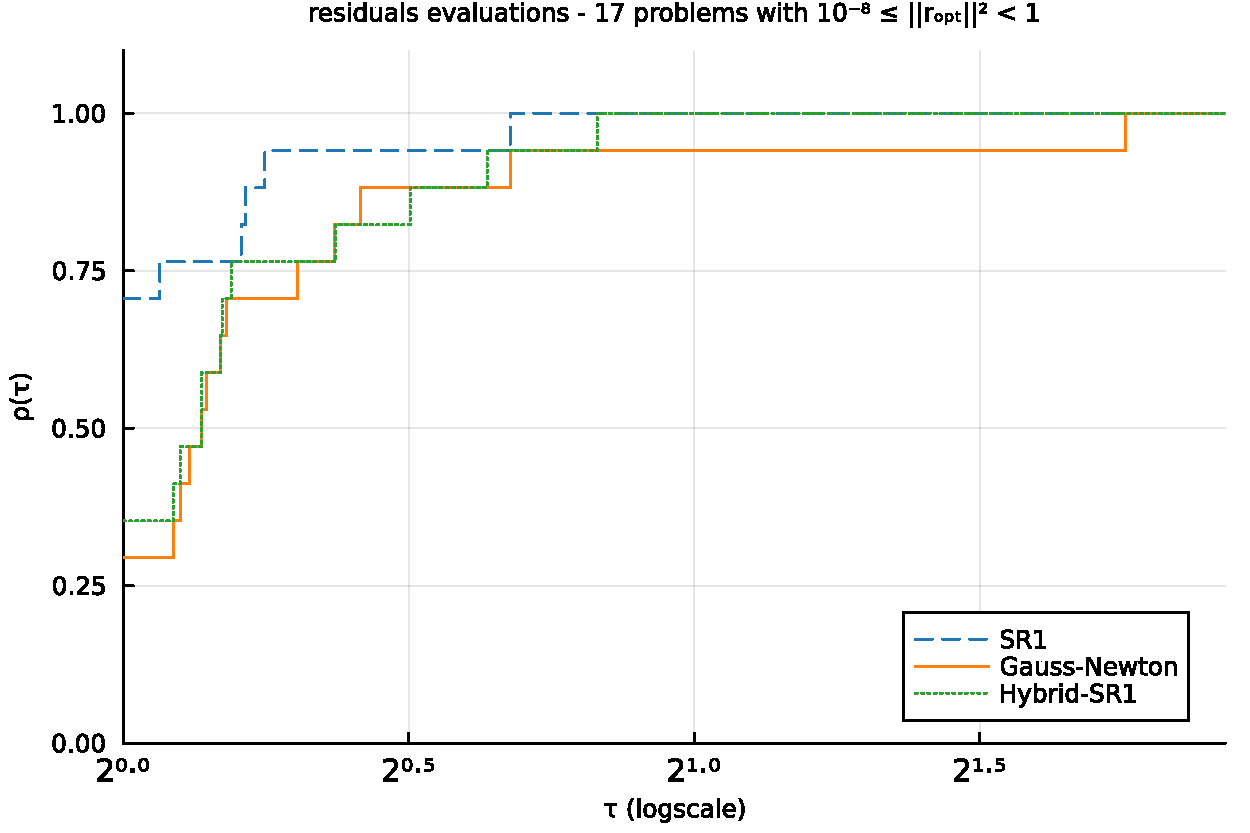
\includegraphics[width=\textwidth]{figures/fig9_small_res_neval_residual}
	\end{subfigure}
	
	\vspace{0.5em}
	
	\begin{subfigure}[b]{0.48\textwidth}
		\centering
		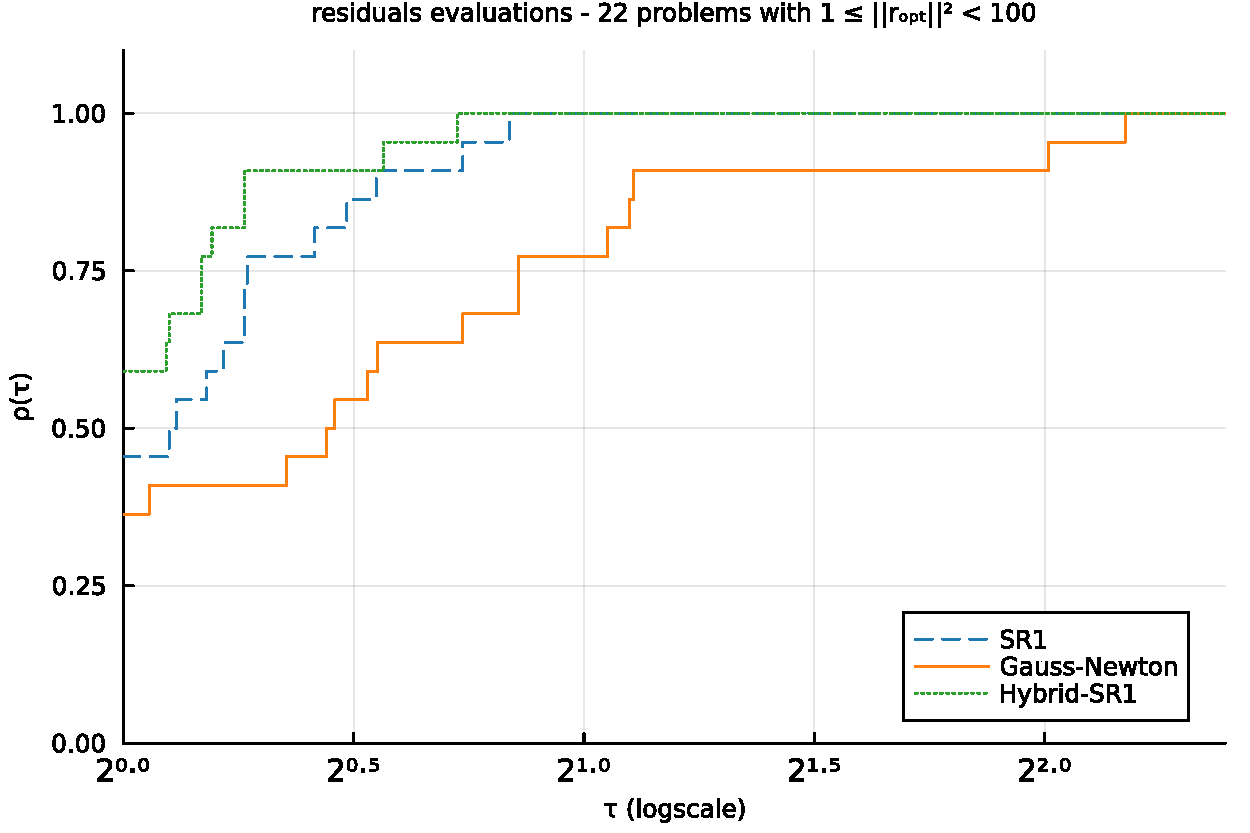
\includegraphics[width=\textwidth]{figures/fig10_medium_res_neval_residual}
	\end{subfigure}
	\hfill
	\begin{subfigure}[b]{0.48\textwidth}
		\centering
		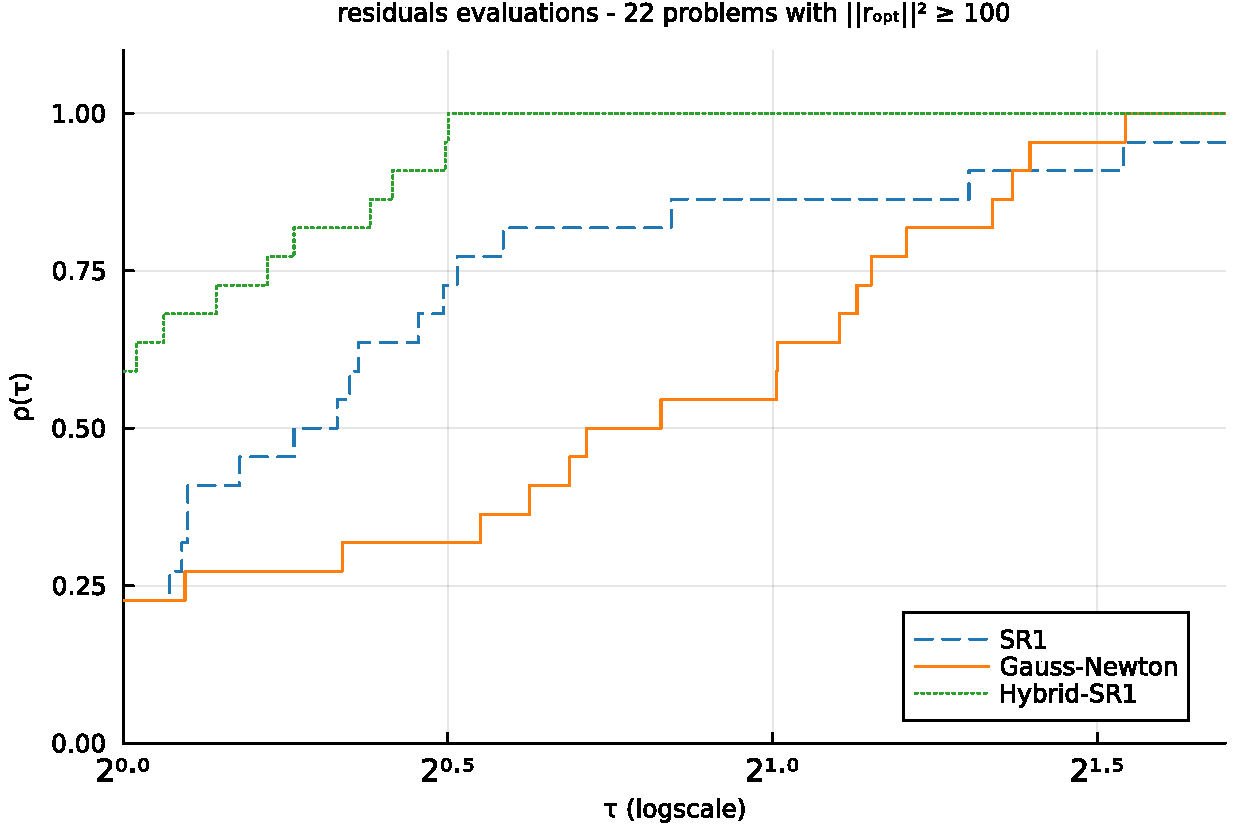
\includegraphics[width=\textwidth]{figures/fig11_large_res_neval_residual}
	\end{subfigure}
	\caption{Performance profiles on the number of residual evaluations, stratified by the squared norm of the residuals at the solution: zero residuals (top left), small residuals (top right), medium residuals (bottom left) and large residuals (bottom right).}
	\label{fig:stratified_reseval}
\end{figure}

The profiles on residual evaluations display a clear trend as the residual magnitude grows. Within a factor $1.5$ of the best count, the GN approximation covers 100\% of the zero-residual instances but only 88\%, 64\% and 36\% of the small-, medium- and large-residual ones, whereas Hybrid-SR1 covers 94\%, 88\%, 96\% and 100\% of the same four groups. The hybrid scheme therefore matches GN when the residuals vanish at the solution -- the regime in which the GN model is asymptotically exact and no correction is needed -- and takes a decisive lead as soon as the residuals are significant. This is precisely the behavior the switching rule is designed to produce.

The plain SR1 update stays close to its hybrid counterpart on the small- and medium-residual instances, and is even ahead on the former, where it is the best variant on 71\% of the instances against 35\% for Hybrid-SR1. The second-order correction is thus beneficial in itself, and the hybrid rule does not always exploit it fully in this intermediate regime. A plausible explanation is that the switching test~\eqref{eq:hybrid_update_strategy} monitors the relative decrease of the augmented Lagrangian $\varphi$, a quantity influenced by both the residual size and the constraint violation, so that nonzero but still small residuals are not always identified as such. In the large-residual regime, by contrast, the hybrid rule is unambiguously the better strategy, and the plain update also suffers there from its failure on HS373.

\begin{figure}[htbp]
	\centering
	\begin{subfigure}[b]{0.48\textwidth}
		\centering
		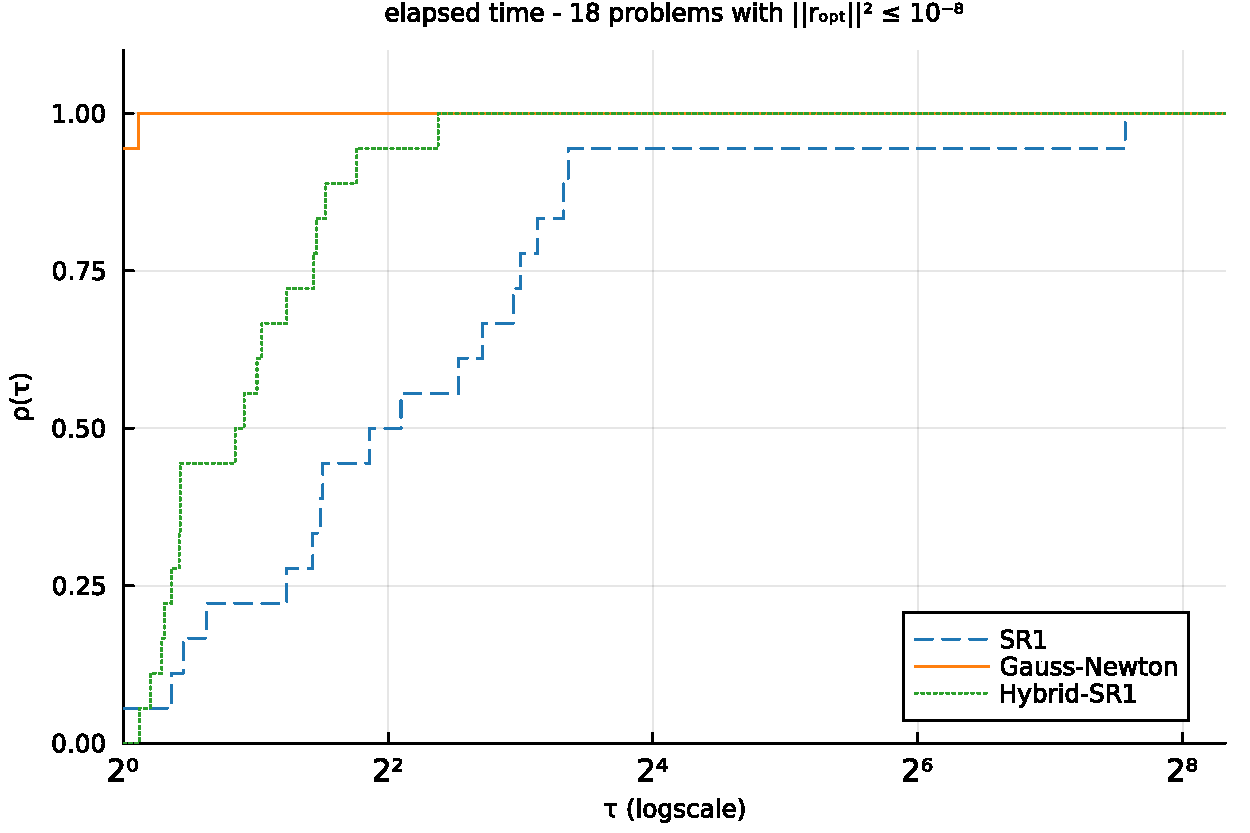
\includegraphics[width=\textwidth]{figures/fig4_zero_res_elapsed_time}
	\end{subfigure}
	\hfill
	\begin{subfigure}[b]{0.48\textwidth}
		\centering
		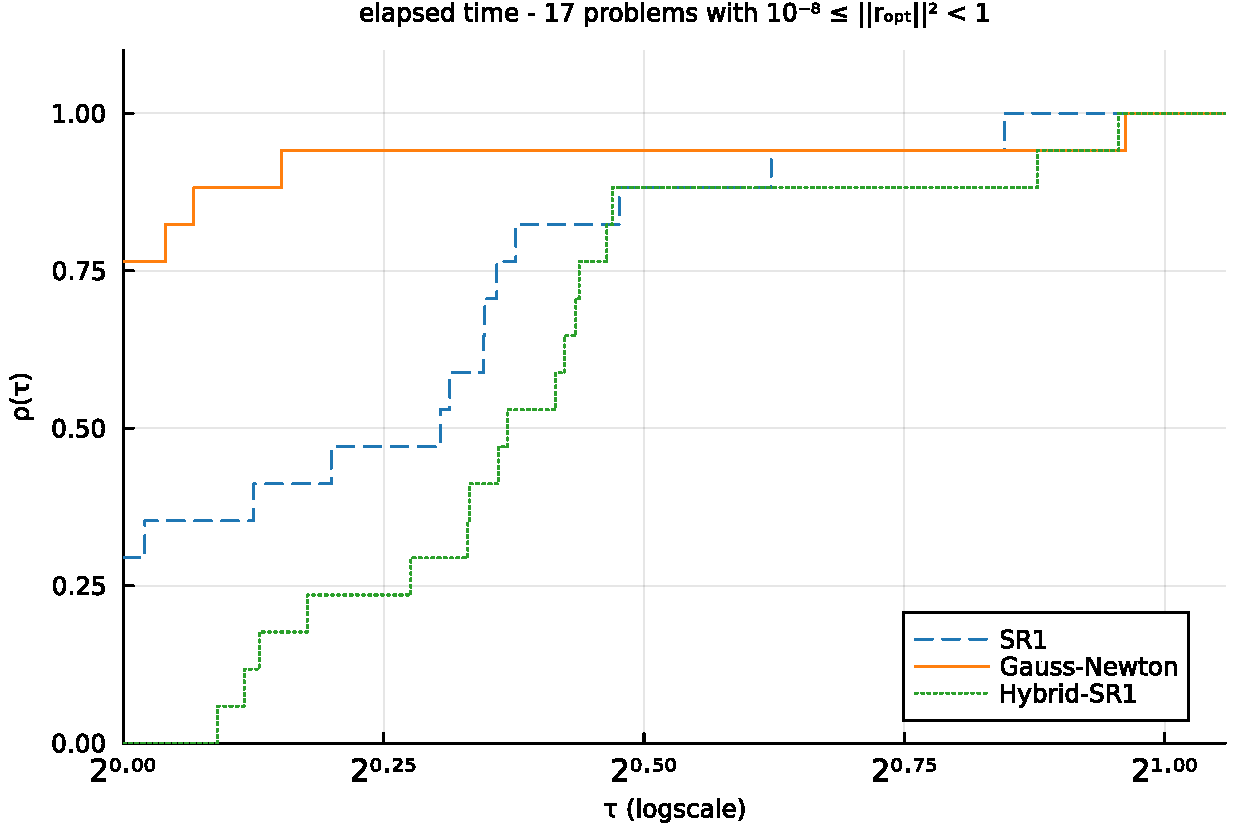
\includegraphics[width=\textwidth]{figures/fig5_small_res_elapsed_time}
	\end{subfigure}
	
	\vspace{0.5em}
	
	\begin{subfigure}[b]{0.48\textwidth}
		\centering
		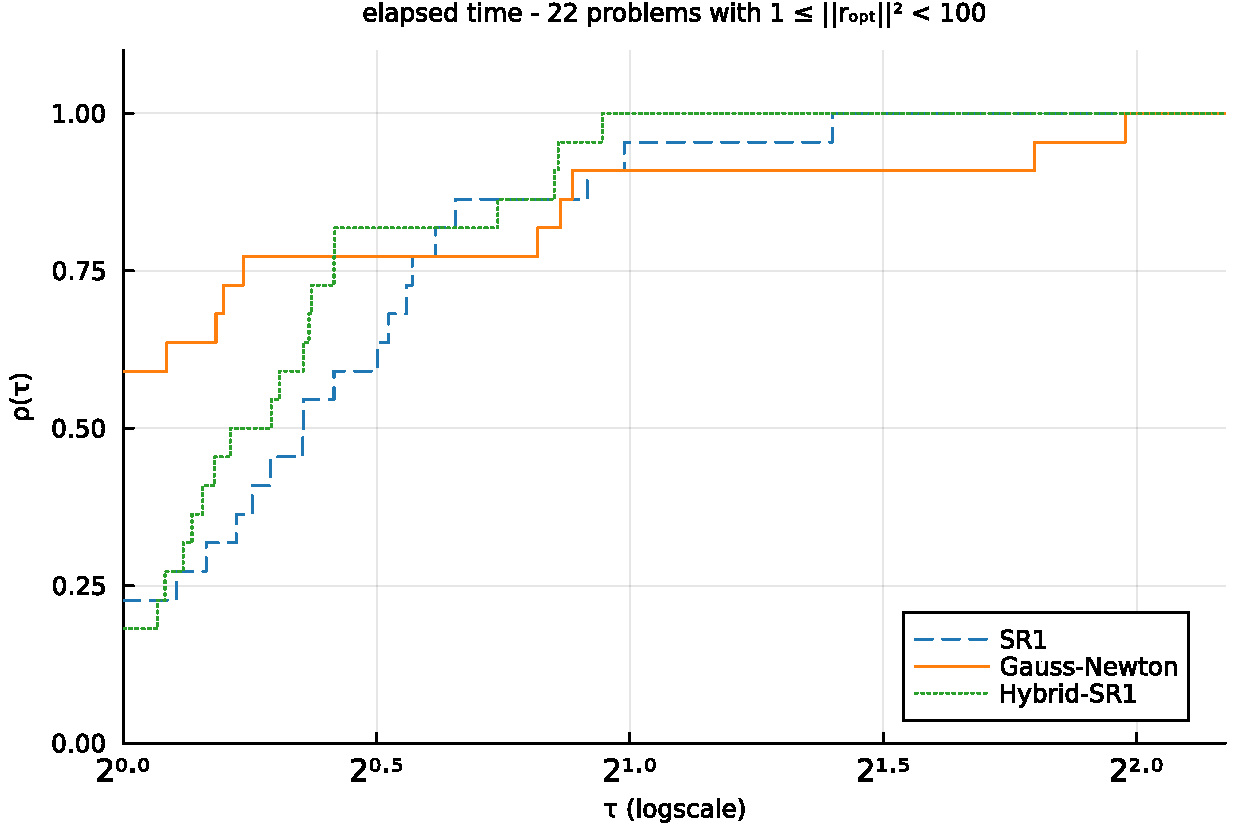
\includegraphics[width=\textwidth]{figures/fig6_medium_res_elapsed_time}
	\end{subfigure}
	\hfill
	\begin{subfigure}[b]{0.48\textwidth}
		\centering
		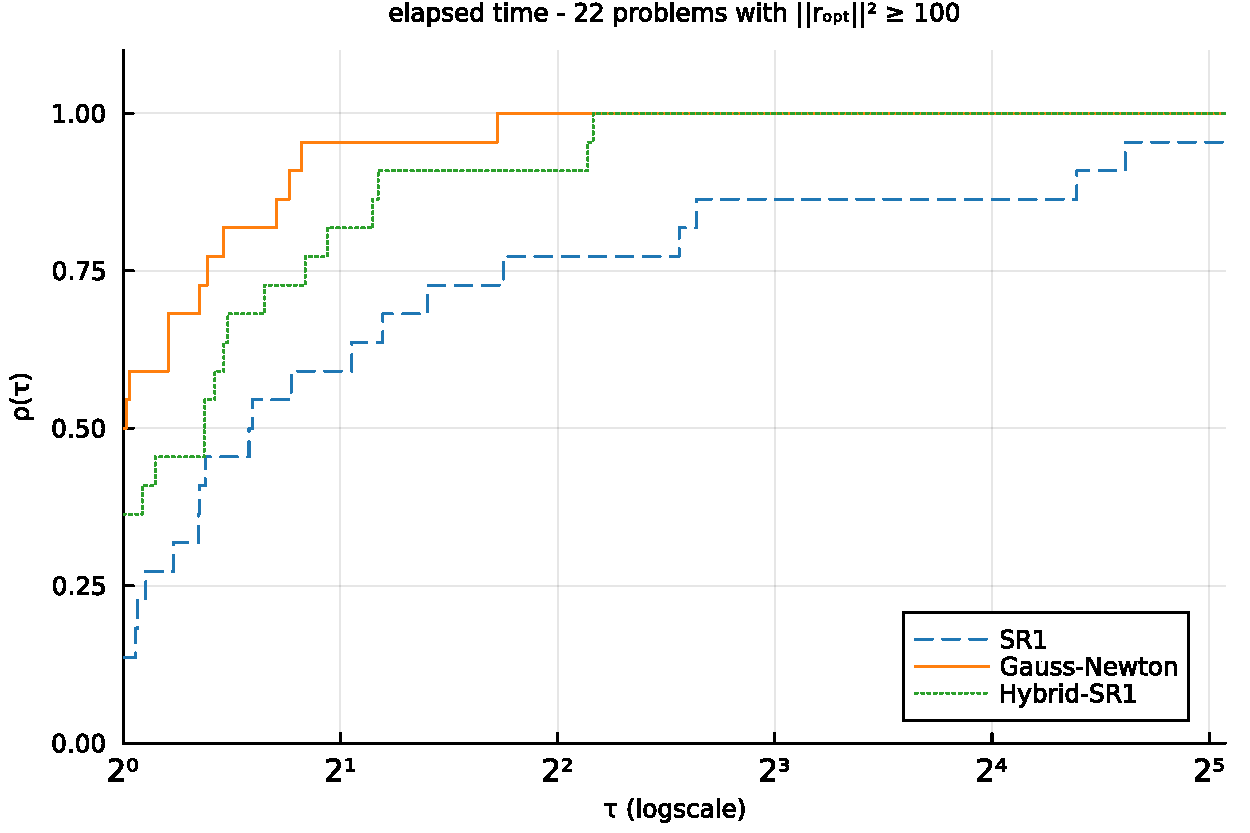
\includegraphics[width=\textwidth]{figures/fig7_large_res_elapsed_time}
	\end{subfigure}
	\caption{Performance profiles on computation time, stratified by the squared norm of the residuals at the solution: zero residuals (top left), small residuals (top right), medium residuals (bottom left) and large residuals (bottom right).}
	\label{fig:stratified_time}
\end{figure}

Computation time, however, favors the GN approximation in every stratum, the gap narrowing as the residuals grow: GN is the fastest variant on 94\%, 76\%, 59\% and 50\% of the zero-, small-, medium- and large-residual instances respectively. The savings in residual evaluations achieved by the hybrid scheme are therefore not compensated by the additional cost of forming and applying a dense second-order correction. This has to be read in light of how the test set is built: all residuals here are evaluated by direct computation and are consequently very cheap. In many applications, and in particular when the residuals come from a simulation code or from the solution of a system of ordinary differential equations, their evaluation is the dominant computational cost. In such settings the profiles of Figure~\ref{fig:stratified_reseval} are the relevant ones, and they show that the structured correction with hybrid switching does reduce the amount of work that actually matters.

Based on these results, we retain the Hybrid-SR1 variant as the best overall strategy for TRAULLS, and use it in the comparisons that follow.

\subsection{Comparison with IPOPT and Percival}\label{subsec:compare_solvers}

We now compare TRAULLS (with the Hybrid-SR1 approximation) against solvers IPOPT~\cite{wachterbiegler:2006} and Percival~\cite{arreckx-etal:2016}. The latter is also an augmented Lagrangian algorithm and has a native Julia implementation. Its inner minimization uses a Julia version of the TRON~\cite{linmore:1999a} algorithm -- part of the \texttt{JSOSolvers.jl} package~\cite{migot-etal:2026}. To benefit from the benchmarking facilities provided by the JuliaSmoothOptimizers (JSO)\footnote{https://jso.dev/} ecosystem, we used the wrapper \texttt{NLPModelsIpopt.jl}~\cite{nlp-models-ipopt-julia}. This allows us to run both solvers on our test set of problems -- all models being encoded in \texttt{NLSProblems.jl}~\cite{nls-problems-julia} -- and export the benchmark metrics using \texttt{SolverBenchmark.jl}~\cite{solver-benchmark-julia}. All solvers share the experimental setup and the tolerances described at the beginning of this section, and were additionally given a maximum CPU time of 10 minutes per instance, a limit consistent with the dimensions of the problems considered.

To make the comparison with IPOPT relevant, we have set the parameters \texttt{nlp\_scaling\_method} = \texttt{none}, \texttt{dual\_inf\_tol} = \texttt{Inf}, \texttt{constr\_viol\_tol} = \texttt{Inf}, \texttt{compl\_inf\_tol} = \texttt{Inf}, \texttt{acceptable\_iter} = \texttt{0} and the maximum number of iterations to 1000. We also set \texttt{hessian\_approximation} = \texttt{limited-memory}, so that IPOPT builds its Hessian model with an L-BFGS update of memory 6 instead of exact second derivatives. This choice makes the comparison meaningful with respect to the derivative information used: like TRAULLS, IPOPT then only requires first-order information about the problem functions and builds curvature from it. For Percival, since it also follows Algorithm~\ref{algo:traulls}, we have set its tolerances and parameters to the same values as ours. We note that Percival, through its TRON inner solver, uses exact Hessian-vector products, and is therefore the only solver of the three that accesses second derivatives.

For these tests, we compare the three solvers against the computation time, the number of residual evaluations and the number of gradient evaluations. Following a criterion also used in~\cite{wachterbiegler:2006} and~\cite{migot-etal:2026}, we removed from the profiles the instances on which all three solvers converge but return objective values whose relative gap between the largest and the smallest exceeds $10^{-2}$, since the solvers then reach distinct local solutions. This concerns nine instances: HS61, HS77, HS264, the instances with $n=100$ of problems 5.1, 5.4, 5.13 and 5.14 from~\cite{lucksanvlcek:1999}, and the instances with $n=500$ and $n=1000$ of problem 5.16 from the same collection. The profiles of Figure~\ref{fig:perf_solvers} are thus built on the remaining 73 instances. On these, TRAULLS and IPOPT converge on every instance, while Percival reaches the maximum CPU time on the two instances of problem 5.11 from~\cite{lucksanvlcek:1999} having $n=500$ and $n=1000$. As a side note, we also ran IPOPT with exact second derivatives, and this configuration failed on two instances, reaching the maximum number of iterations on HS27 and terminating with a restoration phase failure on HS70.

\begin{figure}[htbp]
	\centering
	\begin{subfigure}[b]{0.32\textwidth}
		\centering
		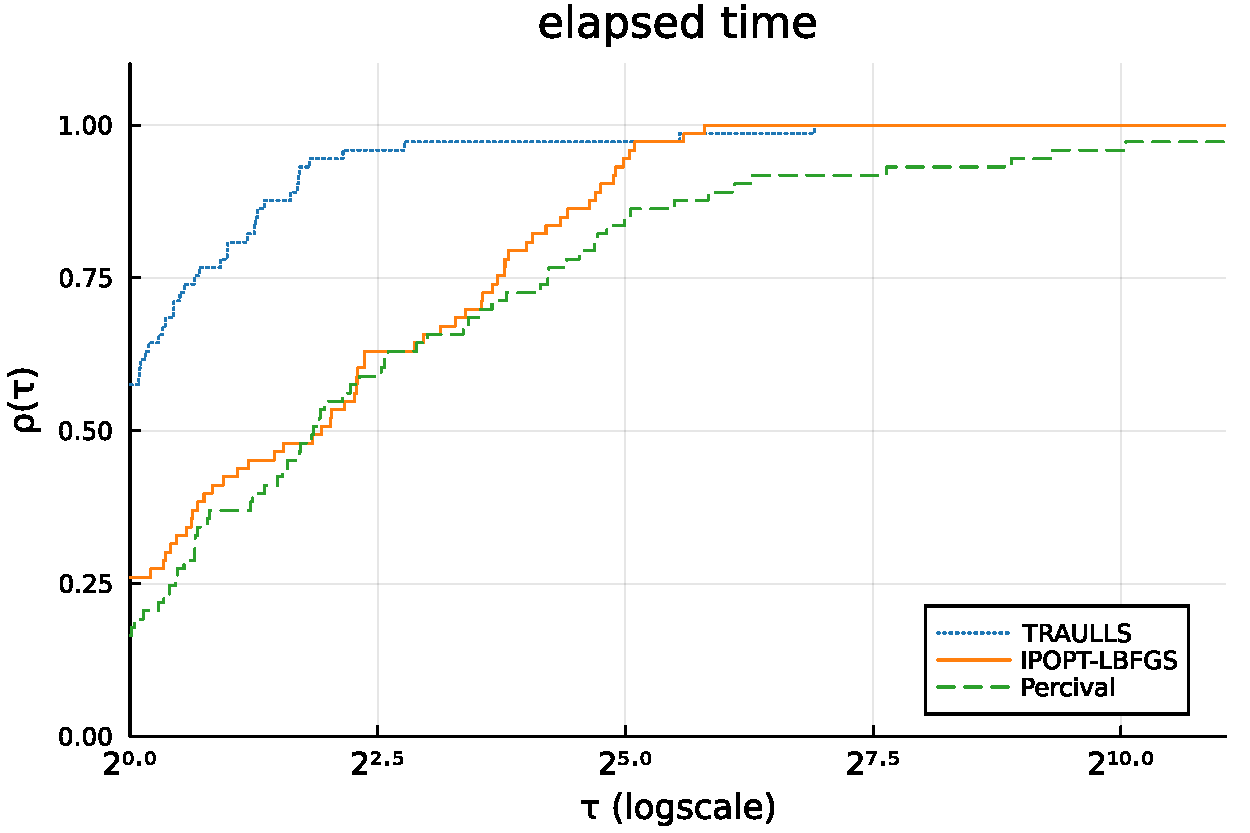
\includegraphics[width=\textwidth]{figures/fig13_traulls_vs_others_elapsed_time}
	\end{subfigure}
	\hfill
	\begin{subfigure}[b]{0.32\textwidth}
		\centering
		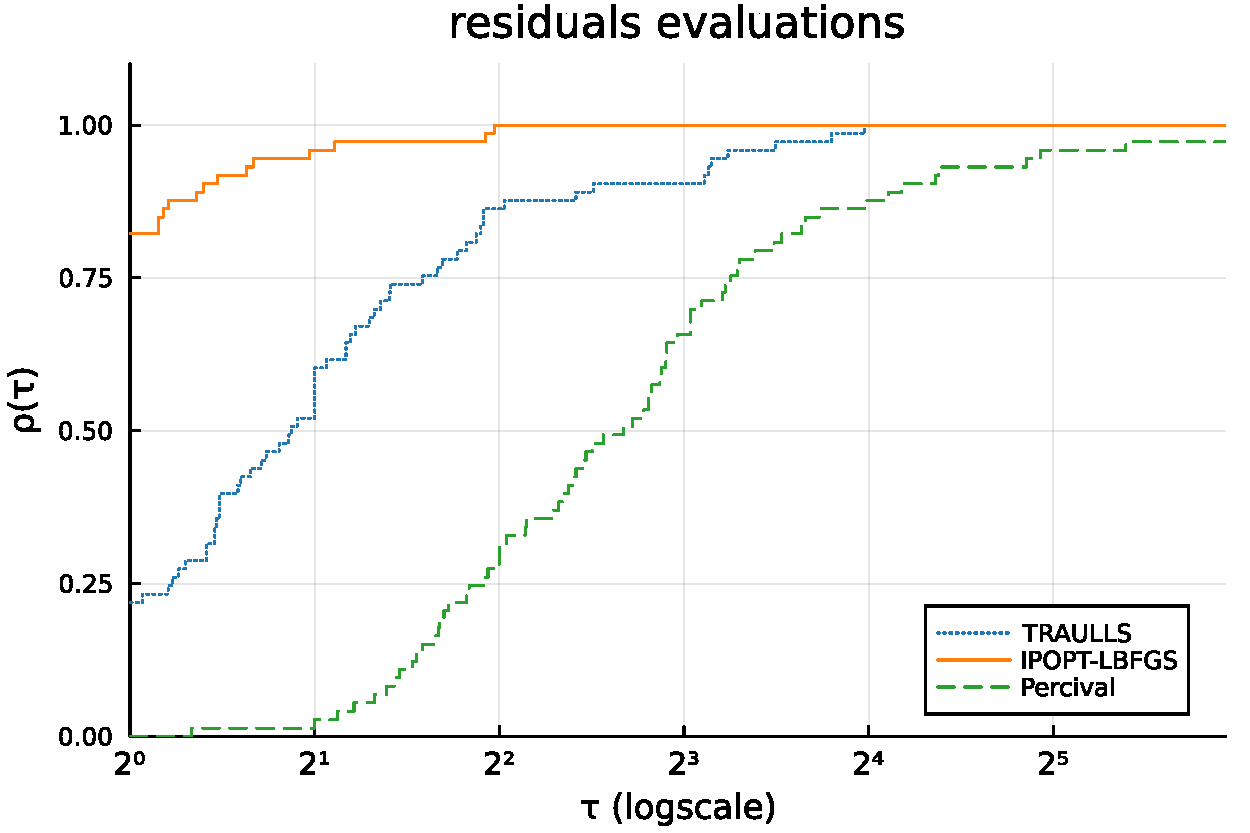
\includegraphics[width=\textwidth]{figures/fig14_traulls_vs_others_neval_residual}
	\end{subfigure}
	\hfill
	\begin{subfigure}[b]{0.32\textwidth}
		\centering
		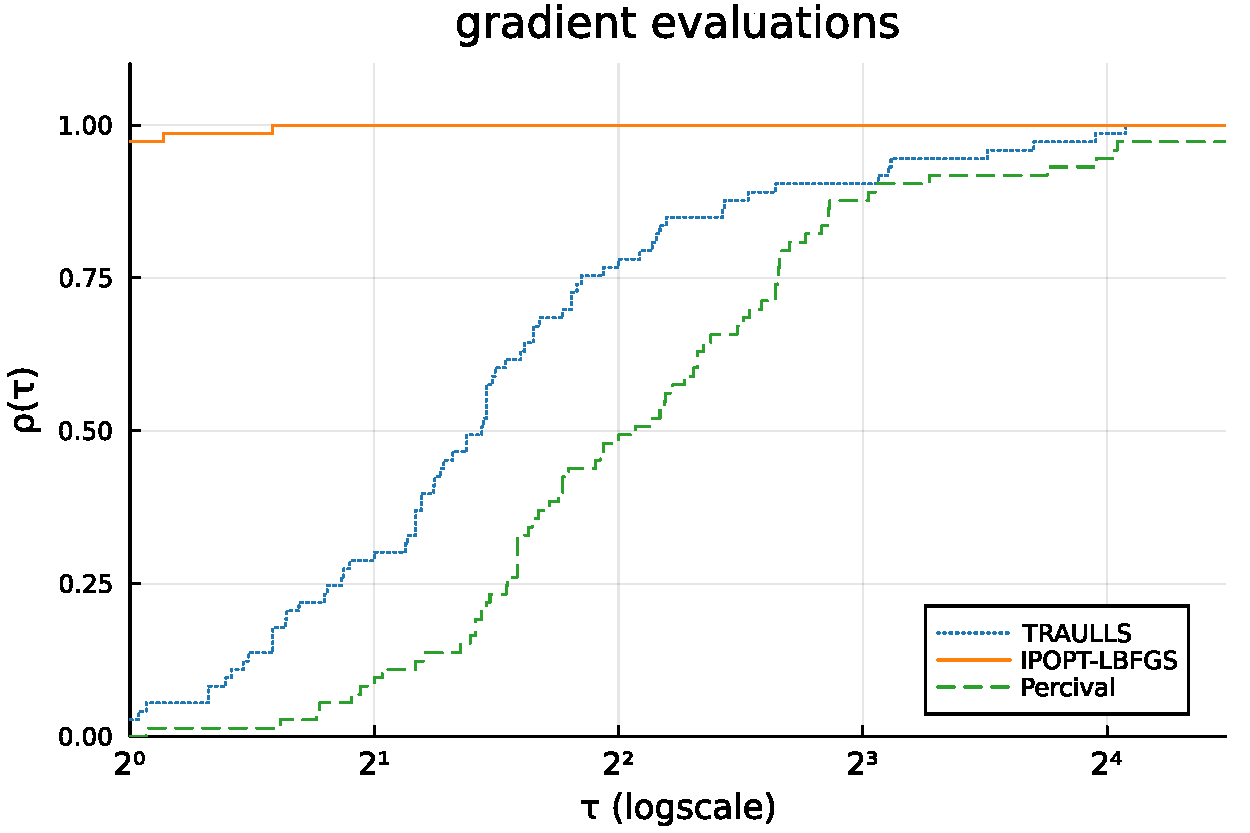
\includegraphics[width=\textwidth]{figures/fig12_traulls_vs_others_neval_grad}
	\end{subfigure}
	\caption{Performance profiles comparing TRAULLS (Hybrid-SR1), IPOPT, and Percival
		on the test set, with respect to computation time (left), residual evaluations (center),
		and gradient evaluations (right).}
	\label{fig:perf_solvers}
\end{figure}

In terms of computation time, TRAULLS is the fastest solver on 58\% of the instances, against 26\% for IPOPT and 16\% for Percival, and it solves 95\% of them within a factor 4 of the best time, against 51\% for IPOPT and 55\% for Percival. Restricting the comparison to IPOPT, TRAULLS is the faster of the two on 73\% of the instances. This advantage is however strongly dependent on the problem size: TRAULLS is faster on 40 of the 41 instances with $n \le 100$, but on only 8 of the 26 instances with $n \ge 500$, where our computation time is on average -- in the geometric mean sense -- $1.79$ times that of IPOPT. The margin observed on the smallest instances should be read with care, as both codes solve them in a few tens of milliseconds at most, with median times of $0.15$ and $1.5$ milliseconds respectively, so that the ratio there mostly reflects a lower fixed cost per solve rather than a difference in the optimization work performed. The large instances are where the gap is algorithmically meaningful, and there the cause is the dense storage and manipulation of the structured second-order correction, whose cost grows quadratically with the number of variables while the rest of the method only involves matrix-vector products. Problem 5.12 from~\cite{lucksanvlcek:1999} with $n=1000$ illustrates this clearly: Hybrid-SR1 solves it in 142 inner iterations against 354 for the GN approximation, yet takes $2.21$ seconds against $1.71$. This is the limitation we discuss in the conclusion, and it is the reason a limited-memory form of the structured update is the natural next step for large-scale problems.

Regarding the evaluation metrics, IPOPT dominates both profiles: it requires the fewest residual evaluations on 82\% of the instances and the fewest gradient evaluations on 97\% of them, where the corresponding figures for TRAULLS are 22\% and 3\%. The gap is larger on gradients than on residuals, and it decomposes into two distinct effects. TRAULLS performs on average $1.91$ times as many residual evaluations as IPOPT, which reflects a genuine difference in the number of steps needed. On top of that, the two methods do not evaluate gradients at the same rate: our trust-region scheme performs $1.16$ gradient evaluations per residual evaluation, against $0.79$ for IPOPT, whose line search reuses a single gradient across the trial points of a backtracking sequence. The product of these two factors, $1.91 \times 1.46 = 2.78$, accounts exactly for the observed ratio of gradient evaluations. Part of the gap is thus structural, inherent to the globalization strategy rather than to the quality of our Hessian model.

These results should be read with the role of each solver in mind. IPOPT is a mature interior-point implementation whose globalization, linear algebra and heuristics differ from ours on every count, and we use it here as an external reference point rather than as the target of our contribution. The comparison that isolates what this work proposes is the one with Percival, which follows the same augmented Lagrangian framework, is run with the same tolerances and parameters, and differs from TRAULLS essentially in that it treats the problem as a generic nonlinear program. There, the advantage of TRAULLS is unambiguous and holds on all three metrics: geometric mean ratios of $0.28$ on computation time, $0.34$ on residual evaluations and $0.69$ on gradient evaluations, TRAULLS being the better of the two on 82\%, 90\% and 79\% of the instances respectively. Unlike the comparison with IPOPT, this advantage does not rest on the smallest instances: restricted to the 32 instances that either solver needs more than ten milliseconds to solve, the ratios become $0.12$, $0.33$ and $0.65$, so the gain grows rather than vanishes as the problems get harder. It is moreover obtained while TRAULLS only approximates second-order information, whereas Percival evaluates exact Hessian-vector products. Within a common algorithmic framework, exploiting the least-squares structure through the Gauss--Newton term and its structured correction therefore leads to a clear improvement, which is the claim this paper makes. That TRAULLS is at the same time faster than a state-of-the-art interior-point code on most of the test set, while requiring more function evaluations than it, situates our implementation as a competitive solver whose remaining bottleneck -- the dense second-order correction on large instances -- is identified and addressable.
